\section{13/11/2024}

We now prove Schur's orthogonality relations. We need some preliminary material. First, recall that 
the matrix $E_{ij}$ is given by 
\[
(E_{ij})_{kl}=\delta_{ik}\delta_{jl},
\qquad
\delta_{xy}=\begin{cases}
    1 & \text{if $x=y$},\\
    0 & \text{otherwise}.
\end{cases}
\]

Let $G$ be a finite group. 
Recall that $L(G)=\{f\colon G\to\C\}$ is a vector space with
\[
    (f+g)(x)=f(x)+g(x),
    \quad
    (\lambda f)(x)=\lambda f(x),
    \quad 
    f,g\in L(G),\,\lambda\in\C,\,x\in G.
\]
The dimension of $L(G)$ is $|G|$. For $x\in G$, 
let 
\[
\delta_x\colon G\to\C,\quad \delta_x(y)=\begin{cases}
    1 & \text{if $x=y$},\\
    0 & \text{otherwise.}
    \end{cases}
\]
Then the set
$\{\delta_x:x\in G\}$ is a basis of $G$. 

If $\alpha\colon G\to\C$ and $\beta\colon G\to\C$ 
are maps, we consider the inner product
\[
\langle\alpha,\beta\rangle=\frac{1}{|G|}\sum_{g\in G}\alpha(g)\overline{\beta(g)}.
\]

If $\rho\colon G\to\GL(V)\simeq\GL_n(\C)$ is a representation of $G$, then
$\rho_g$ is the matrix $(\rho_{ij}(g))$ and hence the character of $\rho$ is given by
\[
\chi_\rho(g)=\sum_{i=1}^n\rho_{ii}(g).
\]



\begin{lemma}
Let $\rho\colon G\to\GL(V)$ and $\psi\colon G\to\GL(W)$ be irreducible representations. Then
$(E_{ki}^\#)_{lj}=\langle\rho_{ij},\psi_{kl}\rangle$.
\end{lemma}

\begin{proof}
  Assume that $\rho$ is unitary. Then $\rho^{-1}_g=\rho_{g^{-1}}=\rho^*_g=\overline{\rho}_g^T$ for all $g\in G$. 
  Thus  
  \begin{align*}
      (E_{ki}^\#)_{lj} &= \frac{1}{|G|}\sum_{g\in G}(\psi_{g^{-1}}E_{ki}\rho_g)_{lj}\\
      &=\frac{1}{|G|}\sum_{g\in G}\sum_{p,q}\psi_{lq}(g^{-1})(E_{ki})_{qp}\rho_{pj}(g)\\
      &=\frac{1}{|G|}\sum_{g\in G}\psi_{lk}(g^{-1})\rho_{ij}(g)\\
      &=\frac{1}{|G|}\sum_{g\in G}\overline{\psi_{kl}(g)}\rho_{ij}(g)=\langle \rho_{ij},\psi_{kl}\rangle.\qedhere
  \end{align*}
\end{proof}

\begin{theorem}[Schur]
\index{Schur's!theorem}
\label{thm:Schur_technical}
    Let $\rho\colon G\to\GL(V)$ and $\psi\colon G\to\GL(W)$ be irreducible representations of a finite group $G$. 
    Then the following statements hold:
    \begin{enumerate}
        \item $\langle\rho_{ij},\psi_{kl}\rangle=0$ if $\rho$ and $\psi$ are not equivalent.
        \item $\displaystyle{\langle\rho_{ij},\rho_{kl}\rangle=\frac{1}{\dim V}\delta_{ik}\delta_{lj}}$.
    \end{enumerate}
\end{theorem}

\begin{proof}
    Let us prove the first claim. Since 
    $\rho$ and $\psi$ 
    are not equivalent, it follows from Schur's lemma that $\Hom_G(V,W)=\{0\}$.
    Thus $E_{ki}^\#\in\Hom_G(V,W)=\{0\}$ (see the comment 
    before the ergodic theorem \ref{thm:ergodic}). 
    
    To prove the second claim, we use the previous lemma:
    \[
    (E_{ki}^\#)_{lj}=\langle\rho_{ij},\rho_{kl}\rangle
    =\frac{1}{\dim V}(\trace E_{ki})\delta_{lj}
    =\frac{1}{\dim V}\delta_{ki}\delta_{lj}.\qedhere
    \]
\end{proof}

Now we can prove Schur's first orthogonality relation.

\begin{theorem}[Schur]
\index{Schur's!theorem}
\index{Schur's!first orthogonality relation}
\label{thm:Schur}
Let $\rho\colon G\to\GL(V)$ and $\psi\colon G\to\GL(W)$ be irreducible representations of a finite group $G$. Then
\[
\langle\chi_\rho,\chi_\psi\rangle=
\begin{cases}
1 & \text{if $\rho\simeq\psi$,}\\
0 & \text{otherwise.}
\end{cases}
\]
\end{theorem}

\begin{proof}
    Let $n=\dim V$ and $m=\dim W$. We compute
    \begin{align*}
        \langle\chi_\rho,\chi_\psi\rangle
        &=\frac{1}{|G|}\sum_{g\in G}\chi_\rho(g)\overline{\chi_\psi}(g)\\
        %&=\frac{1}{|G|}\sum_{g\in G}\sum_{i=1}^n\sum_{j=1}^m\rho_{ii}(g)\overline{\psi_{jj}(g)}\\
        &=\sum_{1=1}^n\sum_{j=1}^m\sum_{g\in G}\frac{1}{|G|}\rho_{ii}(g)\overline{\psi_{jj}(g)}\\
        &=\sum_{1=1}^n\sum_{j=1}^m\langle \rho_{ii},\psi_{jj}\rangle
        =\begin{cases}
            1 & \text{if $\rho\simeq\psi$,}\\
            0 & \text{otherwise.}
        \end{cases}\qedhere
    \end{align*}
\end{proof}

Schur's theorem has several 
corollaries.

\begin{exercise}
Let $G$ be a finite group. 
If $\rho\colon G\to\GL(V)$ is a unitary irreducible representation
of degree $n$, then
\[
\{\sqrt{n}\rho_{ij}:1\leq i,j\leq n\}
\]
is an orthonormal set of size $n^2$.
\end{exercise}

% \begin{corollary}
%     If $\rho\colon G\to\GL(V)$ is an irreducible representaion of degree $n$, then
%     $\{\sqrt{n}\rho_{ij}:1\leq i,j\leq n\}$ is an orthonormal set.
% \end{corollary}



% If $G$ is a finite group, let $K(G)$ be the number of conjugacy classes of $G$. 
% We want to know how many irreducible representations are there. For that purpose, 
% we need to study the space of class functions. 


\begin{corollary}
     A finite group has finitely many classes of irreducible representations. 
\end{corollary}

\begin{proof}
     Let $G$ be a finite group. 
     Every isomorphism class of representations of $G$ contains a unitary representation (Corollary \ref{cor:consequences}). 
     Since $\dim L(G)=|G|$, every linearly independent set 
     of vectors from $L(G)$ has at most $|G|$ elements. By
     Schur's theorem \ref{thm:Schur}, the entries
     of inequivalent unitary representations of $G$ 
     form an orthogonal set of non-zero vectors of $L(G)$. Thus
     there are at most $|G|$ equivalence classes of irreducible
     representations. 
%     it follows that $G$ admits $\leq|G|$ equivalence classes of irreducible representations. Let
%     $\rho_1,\dots\rho_r$ be the representatives of the isomorphism classes of the 
%    irreducible representations of $G$. At the moment, we do not know whether $r$ is finite. 
%    For each $k$ let $n_k=\deg\rho_k$. Since
%     the $n_1^2+\cdots n_r^2$ maps $\sqrt{n_k}(\rho_k)_{ij}$, $1\leq k\leq r$, $1\leq i,j\leq n_k$,
%     form a non-zero orthonormal set of $L(G)$, it follows that
%     $r\leq n_1^2+\cdots+ n_r^2\leq|G|$.
\end{proof}

Let $G$ be a finite group. Since $G$ has only finitely many non-equivalent 
irreducible representation, we will often say
that 
\[
\rho_1,\dots,\rho_r
\]
are \emph{the} irreducible representations of $G$, where it is assumed that
the $\rho_i$ form a complete set of 
representatives of irreducible representations of $G$. For each $i$ we write
$\chi_i=\chi_{\rho_i}$. The set of irreducible characters will be denoted
by 
\[
\Irr(G)=\{\chi_1,\dots,\chi_r\}.
\]

\begin{definition}
\index{Class function}
	Let $G$ be a group and 
	$f\colon G\to\C$ be a map. Then $f$ is a \emph{class function} if
	$f(g)=f(hgh^{-1})$ for all $g,h\in G$. 	
\end{definition}

Characters are class functions. 


If $g\in G$, the \emph{conjugacy class} of $g$ in $G$ 
is the set $\{xgx^{-1}:x\in G\}$. Note that two conjugacy classes are either equal or disjoint. Moreover, 
every group is a disjoint union of its conjugacy classes. 
For example, the conjugacy classes of the group $\Sym_3$ are  
$\{\id\}$, $\{(12),(13),(23)\}$ and $\{(123),(132)\}$. Thus $\Sym_3$ has three conjugacy classes. 

Let $C(G)$ be the subspace of $L(G)$ of class functions. 

\begin{proposition}
    Let $G$ be a finite group. Then $\dim C(G)=K(G)$, the number of conjugacy classes of $G$.
\end{proposition}

\begin{proof}
If $C$ is a conjugacy class, 
then 
\[
\delta_C\colon G\to\C,\quad
\delta_C(x)=\begin{cases}
    1 & \text{if $x\in C$,}\\
    0 & \text{otherwise,}
\end{cases}
\]
is a class function.  
It is enough to prove that the 
set $\{\delta_C:C\text{ is a conjugacy class of $G$}\}$ is a basis of $C(G)$.  It is a generating set
because each $f$ can be written as 
\[
f=\sum_{C}f(C)\delta_C.
\]
The $\delta_C$ are linearly independent because they are orthogonal: 
If $C$ and $D$ 
are conjugacy classes of $G$, then 
\[
\langle\delta_C,\delta_D\rangle=\frac{1}{|G|}\sum_{x\in G}\delta_C(x)\overline{\delta_D(x)}
=\begin{cases}
|C|/|G| & \text{if $C=D$},\\
0 & \text{otherwise}.
\end{cases}
\]
From this the claim follows. 
\end{proof}


\begin{corollary}
    Let $G$ be a finite group. There are at most $K(G)$ equivalence classes of irreducible representations of $G$.
\end{corollary}

\begin{proof}
    Non-equivalent representations have different characters. 
    Irreducible characters 
    form an orthonormal set, thus they are linearly 
    independent. Since irreducible characters
    are class functions (that is, they are constant on conjugacy classes), 
    it follows that there are at most $K(G)$ irreducible different characters.  
\end{proof}

Let $m\in\Z_{>0}$. If $V$ is a vector space, we 
write \[
mV=V\oplus\cdots\oplus V\quad\text{($m$-times)}.
\]
Similarly,
if $\rho$ is a representation, 
we write 
\[
m\rho=\rho\oplus\cdots\oplus\rho\quad\text{($m$-times)}.
\]

\begin{theorem}
    Let $\rho_1,\dots,\rho_r$ be the irreducible representations of a finite group $G$. If 
	\[ 
    \rho=\sum_{j=1}^rm_j\rho_j,
    \]
    where $m_1,\dots m_r\in\Z_{\geq0}$, then
    $m_i=\langle \chi_\rho,\chi_i\rangle$ for all $i\in\{1,\dots,r\}$. 
\end{theorem}

\begin{proof}
    Write $\chi_\rho=\sum_{j=1}^rm_j\chi_j$. Then
    \[
    \langle\chi_\rho,\chi_i\rangle=\sum_{j=1}^rm_j\langle\chi_j,\chi_i\rangle=m_i
    \]
    for all $i\in\{1,\dots,r\}$.
\end{proof}

The theorem states that the decomposition of a representation $\rho$ into irreducibles 
is unique and is determined (up to equivalence) by its character.

\begin{corollary}
    A representation $\rho$ of a finite group with character $\chi_\rho$ is irreducible if and only if $\langle\chi_\rho,\chi_\rho\rangle=1$.
\end{corollary}

\begin{proof}
    We first decompose $\rho$ as a sum of irreducibles, say \[
    \rho=\sum_{j=1}^rm_j\rho_j
    \]
    with $m_1,\dots,m_r\geq0$. Then
    $\langle\chi_\rho,\chi_\rho\rangle=\sum_{j=1}^rm_j^2$. Now $\langle\chi_\rho,\chi_\rho\rangle=1$ if and only if
    there is exactly one $j$ such that $m_j=1$ and $m_i=0$ for all $i\ne j$.  
\end{proof}

\begin{exercise}
    Let $G$ and $H$ be finite groups. 
    If $\rho\colon H\to\GL(V)$ is an irreducible
    representation of $H$ and 
    $f\colon G\to H$ is a surjective group homomorphism, then the composition $\rho f\colon G\to\GL(V)$ is an irreducible representation. 
\end{exercise}

Recall that the left regular representation of a finite group $G$
is the group homomorphism $L\colon G\to \GL(V)$, where $V$ is the complex vector space
with basis $\{g:g\in G\}$ and $L_g(x)=gx$ for all $g,x\in G$. 

\begin{theorem}
    Let $G$ be a finite group and $L$ be its regular representation. 
    Then $L=\sum_{j=1}^rn_j\rho_j$, where $n_j=\deg\rho_j$. 
\end{theorem}

\begin{proof}
    Let $G=\{g_1,\dots,g_n\}$, $n=|G|$. If $g\in G$, since
    $L_g(g_i)=gg_i$ for all $i$, 
    the matrix of $L_g$ in the basis $\{g_1,\dots,g_n\}$ is then
    \begin{gather*}
    (L_g)_{ij}=\begin{cases}
        1 & \text{if $g_i=gg_j$},\\
        0 & \text{otherwise}.
    \end{cases}
    \shortintertext{Then}
    \chi_L(g)=\trace(L_g)=\sum_{i=1}^n(L_g)_{ii}=\begin{cases}
        |G| & \text{if $g=1$},\\
        0 & \text{otherwise}.
    \end{cases}
    \end{gather*}
    In particular, 
    \[
    \langle\chi_L,\chi_i\rangle=\frac{1}{|G|}\sum_{g\in G}\chi_L(g)\overline{\chi_i(g)}
    =\frac{1}{|G|}|G|\overline{\chi_i(1)}=n_i
    \]
    for all $i\in\{1,\dots,n\}$. 
\end{proof}

Now several corollaries. 

\begin{corollary}
    Let $G$ be a finite group and $\rho_1,\dots,\rho_r$ be the irreducible representations of $G$. 
    For each $k$ let $n_k=\deg\rho_k$. The following statements hold:
    \begin{enumerate}
        \item $|G|=n_1^2+\cdots+n_r^2$.
        \item $\{\sqrt{n_k}(\rho_k)_{ij}:1\leq k\leq r,\,1\leq i,j\leq n_k\}$
            is an orthonormal basis of $L(G)$. 
        \item $r$ is equal to the number of conjugacy classes of $G$. 
    \end{enumerate}
\end{corollary}

\begin{proof}
    Since $\chi_L=\sum_{j=1}^rn_j\chi_j$, the first claim follows. 
    The second claim follows from the orthogonality relations. Let us prove the third claim. Let $f\in C(G)$ and write $f$ 
    as a linear combination of the $(\rho_k)_{ij}$, say
    \[
    f=\sum_{i,j,k}\lambda_{ijk}(\rho_k)_{ij},\quad\lambda_{ijk}\in\C.
    \]
    If $x\in G$, then 
    \begin{align*}
    f(x)&=\frac{1}{|G|}\sum_{g\in G}f(g^{-1}xg)\\
    &=\frac{1}{|G|}\sum_{g\in G}\sum_{i,j,k}\lambda_{ijk}(\rho_k)_{ij}(g^{-1}xg)
    =\sum_{i,j,k}\lambda_{ijk} \frac{1}{|G|}\sum_{g\in G}(\rho_k)_{ij}(g^{-1}xg). 
    \end{align*}
    Let $T=(\rho_k)_x=\rho_k(x)\colon V\to V$. Then
    \[
    T^{\#}=\frac{1}{|G|}\sum_{g\in G}(\rho_k)_{g^{-1}}(\rho_k)_x(\rho_k)_g
    =\frac{1}{|G|}\sum_{g\in G}(\rho_k)(g^{-1}xg)
    =\frac{1}{n_k}\chi_k(x)\id
    \]
    by the Ergodic theorem and because 
    $\rho_k$ is a group homomorphism. Thus 
    \[
    f(x)=\sum_{i,j,k}\lambda_{ijk} \left((\rho_k)_x\right)_{ij}
    =\sum_{i,j,k}\lambda_{ijk}\frac{1}{n_k}\chi_k(x)\delta_{ij}
    =\sum_{i,k}\lambda_{iik}\frac{1}{n_k}\chi_k(x).\qedhere 
    \]
    This implies that $\dim C(G)\leq r$ and the claim follows. 
\end{proof}

In the following exercise, the reader is asked to prove the second 
Schur's orthogonality relation. 

\begin{exercise}
    Let $G$ be a finite group and 
    $C$ and $D$ be conjugacy classes of $G$. If $g\in C$ and $h\in D$, then
    \[
    \sum_{\chi\in\Irr(G)}\chi(g)\overline{\chi(h)}=
    \begin{cases}
    |G|/|C| & \text{if $C=D$},\\
    0 & \text{otherwise}.
    \end{cases}
    \]
\end{exercise}

\subsection{Examples}

Let $G$ be a finite group and $\chi_1,\dots,\chi_r$ be the irreducible characters of $G$. Without loss of generality
we may assume that $\chi_1$ is the trivial character, i.e. $\chi_1(g)=1$ for all $g\in G$. 
Recall that $r$ is the number of conjugacy classes of $G$. Each $\chi_j$ is constant on conjugacy classes. 
The \emph{character table} of 
$G$ is given by 
\begin{center}
\begin{tabular}{|c|cccc|}
\hline 
 & $1$ & $k_{2}$ & $\cdots$ & $k_{r}$\tabularnewline
 & $1$ & $g_{2}$ & $\cdots$ & $g_{r}$\tabularnewline
\hline 
$\chi_{1}$ & $1$ & $1$ & $\cdots$ & $1$\tabularnewline
$\chi_{2}$ & $n_{2}$ & $\chi_{2}(g_{2})$ & $\cdots$ & $\chi_{2}(g_{r})$\tabularnewline
$\vdots$ & $\vdots$ & $\vdots$ & $\ddots$ & $\vdots$\tabularnewline
$\chi_{r}$ & $n_{r}$ & $\chi_{r}(g_{2})$ & $\cdots$ & $\chi_{r}(g_{r})$\tabularnewline
\hline
\end{tabular}
\end{center}
where the $n_j$ are the degrees of the irreducible representations of $G$ and each $k_j$ is 
the size of the conjugacy class of the element $g_j$. By convention, the character table
contains not only the values of the irreducible characters of the group. 

\begin{example}
	Sea $G=\langle g:g^4=1\rangle$ 
	be the cyclic group of order four. The character table of $G$ is given by
	\begin{center}
		\begin{tabular}{|c|cccc|}
			\hline 
			& 1 & 1 & 1 & 1\tabularnewline
			& $1$ & $g$ & $g^2$ & $g^{3}$\tabularnewline
			\hline 
			$\chi_{1}$ & $1$ & $1$ & $1$ & $1$\tabularnewline
			$\chi_{2}$ & $1$ & $\lambda$ & $\lambda^2$ & $\lambda^{3}$\tabularnewline
			$\chi_{3}$ & $1$ & $\lambda^2$ & $\lambda^4$ & $\lambda^{2}$\tabularnewline
			$\chi_{4}$ & $1$ & $\lambda^{3}$ & $\lambda^{2}$ & $\lambda$\tabularnewline
			\hline
		\end{tabular}
	\end{center}
% Let us see how to see this calculation in the computer:
% \begin{lstlisting}
% gap> C4 := CyclicGroup(4);;                       
% gap> T := CharacterTable(C4);;
% gap> Display(T);
% CT1

%      2  2  2  2  2

%       1a 4a 2a 4b

% X.1     1  1  1  1
% X.2     1 -1  1 -1
% X.3     1  A -1 -A
% X.4     1 -A -1  A

% A = E(4)
%   = Sqrt(-1) = i
% \end{lstlisting}
% We need some remarks
% \begin{enumerate}
%     \item The symbol \lstinline{E(4)} denotes a primitive fourth root of 1.
%     \item The function \lstinline{CharacterTable} computes some more information, not only the character table of the group. 
%     esta función calcula algunas otras cosas. Por ejemplo:
% \end{enumerate}
% \begin{lstlisting}
% gap> OrdersClassRepresentatives(T);
% [ 1, 4, 2, 4 ]
% gap> SizesCentralizers(T);
% [ 4, 4, 4, 4 ]
% gap> SizesConjugacyClasses(T);
% [ 1, 1, 1, 1 ]
% \end{lstlisting}
\end{example}

\begin{exercise}
	Let $n\in\Z_{>0}$ be such that $n\geq2$. Let 
$C_n=\langle g:g^n=1\rangle$ be the cyclic group of order $n$.
\begin{enumerate}
    \item Prove that the maps  
        $\chi_i\colon C_n\to\C^\times$, $g^k\mapsto e^{2\pi ik/n}$, where $i\in\{0,1,\dots,n-1\}$, 
        are the irreducible representations of $C_n$. 
    \item Let $\lambda$ be a primitive root of 1 of order $n$. Prove that 
        the character table of $C_n$ of order $n$ is given by 
	\begin{center}
		\begin{tabular}{|c|ccccc|}
			\hline 
			& 1 & 1 & 1 & $\cdots$ & 1\tabularnewline
			& $1$ & $g$ & $g^2$ & $\cdots$ & $g^{n-1}$\tabularnewline
			\hline 
			$\chi_{1}$ & $1$ & $1$ & $1$ & $\cdots$ & $1$\tabularnewline
			$\chi_{2}$ & $1$ & $\lambda$ & $\lambda^2$ & $\cdots$ & $\lambda^{n-1}$\tabularnewline
			$\chi_{3}$ & $1$ & $\lambda^2$ & $\lambda^4$ & $\cdots$ & $\lambda^{n-2}$\tabularnewline
			$\vdots$ & $\vdots$ & $\vdots$ & $\vdots$ & $\ddots$ & $\vdots$\tabularnewline
			$\chi_{n}$ & $1$ & $\lambda^{n-1}$ & $\lambda^{n-2}$ & $\cdots$ & $\lambda$\tabularnewline
			\hline
		\end{tabular}
	\end{center}
\end{enumerate}
\end{exercise}

\begin{exercise}
    Let $A$ and $B$ be finite abelian groups. We write $\Irr(A)=\{\rho_1,\dots,\rho_r\}$ and 
    $\Irr(B)=\{\phi_1,\dots,\phi_s\}$. Prove
    that the maps 
    \[
    \varphi_{ij}\colon A\times B\to\C^\times,\quad
    (a,b)\mapsto\rho_i(a)\phi_j(b),
    \]
    where $i\in\{1,\dots,r\}$ and $j\in\{1,\dots,s\}$, are the irreducible representations of $A\times B$. 
\end{exercise}

Let us show a particular example of the previous exercise. 

\begin{example}
	The character table of the group $C_2\times C_2=\{1,a,b,ab\}$ is 
	\begin{center}
		\begin{tabular}{|c|rrrr|}
			\hline 
			& 1 & 1 & 1 & 1\tabularnewline
			& $1$ & $a$ & $b$ & $ab$\tabularnewline
			\hline 
			$\chi_{1}$ & $1$ & $1$ & $1$ & $1$\tabularnewline
			$\chi_{2}$ & $1$ & $1$ & $-1$ & $-1$\tabularnewline
			$\chi_{3}$ & $1$ & $-1$ & $1$ & $-1$\tabularnewline
			$\chi_{4}$ & $1$ & $-1$ & $-1$ & $1$\tabularnewline
			\hline
		\end{tabular}
	\end{center}
% 	Let us do this by computer:
% \begin{lstlisting}
% gap> Display(CharacterTable(AbelianGroup([2,2])));
% CT2

%      2  2  2  2  2

%       1a 2a 2b 2c

% X.1     1  1  1  1
% X.2     1 -1  1 -1
% X.3     1  1 -1 -1
% X.4     1 -1 -1  1
% \end{lstlisting}
\end{example}

%Clearly, the order in which the computer returns the irreducible characters is not %necessarily the same we used! 

\begin{example}
	The symmetric group $\Sym_3$ has three conjugacy classes. The representatives are 
	$\id$, $(12)$ and $(123)$. There are three irreducible representations. We already found all the irreducible characters! 
	The character table of $\Sym_3$ is given by 
	\begin{center}
		\begin{tabular}{|c|rrr|}
			\hline
			& $1$ & $3$ & $2$\tabularnewline
			& $1$ & $(12)$ & $(123)$ \tabularnewline
			\hline 
			$\chi_{1}$ & $1$ & $1$ & $1$\tabularnewline
			$\chi_{2}$ & $1$ & $-1$ & $1$ \tabularnewline
			$\chi_{3}$ & $2$ & $0$ & $-1$ \tabularnewline
			\hline
		\end{tabular}
	\end{center}
	Let us recall how this table was computed. Degree-one irreducibles were easy to compute. 
	To compute the third row of the table one possible approach is to use
	the irreducible representation  
	\[
	(12)\mapsto \begin{pmatrix}-1&1\\0&1\end{pmatrix},
	\quad
	(123)\mapsto \begin{pmatrix}0&-1\\1&-1\end{pmatrix}.
	\]
    Then	
    \begin{align*}
		&\chi_3\left( (12) \right)=\trace\begin{pmatrix}-1&1\\0&1\end{pmatrix}=0,\\
		&\chi_3\left( (123) \right)=\chi_3\left( (12)(23)\right)=\trace\begin{pmatrix}0&-1\\1&-1\end{pmatrix}=-1.
	\end{align*}

	We should remark that the irreducible representation mentioned is not really needed to
	compute the third row of the character table. We can, for example, use the regular
	representation $L$. The character of $L$ is given by 
	\[
		\chi_L(g)=\begin{cases}
			6 & \text{si $g=\id$},\\
			0 & \text{si $g\ne\id$}.
		\end{cases}
	\]
	The equality $0=\chi_L\left( (12) \right)=1-1+2\chi_3( (12))$ implies that 
	$\chi_3( (12))=0$ and the equality 
    \[ 
    0=\chi_L( (123))=1+1+2\chi_3( (123))
    \]
	implies that $\chi_3\left( (123) \right)=-1$. 

	Another approach uses the orthogonality relations. We need to compute $\chi_3( (12) )$ and $\chi_3( (123))$. 
	Let $a=\chi_3( (12) )$ and $b=\chi_3( (123))$. Then 
    we get that $a=0$ and $b=-1$. We just need to solve  
	\begin{align*}
		0&=\langle \chi_3,\chi_1\rangle=\frac16(2+3a+2b),\\
		0&=\langle \chi_3,\chi_2\rangle=\frac16(2-3a+2b).
	\end{align*}
	
% 	Let us use the computer:
% 	\begin{lstlisting}
% gap> S3 := SymmetricGroup(3);;
% gap> T := CharacterTable(S3);;
% gap> Display(T);
% CT3

%      2  1  1  .
%      3  1  .  1

%       1a 2a 3a
%     2P 1a 1a 3a
%     3P 1a 2a 1a

% X.1     1 -1  1
% X.2     2  . -1
% X.3     1  1  1
% \end{lstlisting}
% As we did before, some extra information was computed:
% \begin{lstlisting}
% gap> SizesConjugacyClasses(T);
% [ 1, 3, 2 ]
% gap> SizesCentralizers(T);
% [ 6, 2, 3 ]
% gap> SizesConjugacyClasses(T);
% [ 1, 3, 2 ]
% gap> OrdersClassRepresentatives(T);
% [ 1, 2, 3 ]
% \end{lstlisting}
\end{example}

%A challenging exercise: 
\begin{exercise}
Compute the character table of $\Sym_4$. 
\end{exercise}

\begin{example}
	We now compute the character table of the alternating group $\Alt_4$. This group has $12$ 
	elements and four conjugacy classes.
	\begin{center}
		\begin{tabular}{c|cccc}
			representative & $\id$ & $(123)$ & $(132)$ & $(123)$\tabularnewline
			\hline
			size & $1$ & $4$ & $4$ & $3$ 
		\end{tabular}
	\end{center}
	Since 
 \[
 [\Alt_4,\Alt_4]=\{\id,(12)(34),(13)(24),(14)(23)\},
 \]
	the quotient $\Alt_4/[\Alt_4,\Alt_4]$ has three elements. Thus $\Alt_4$ has three degree-one irreducibles and
	an irreducible character of degree three. Let 
	$\omega=\exp(2\pi i/3)$ be a primitive cubic root of 1. If $\chi$
	is a non-trivial degree-one character, then 
	$\chi\left( (123) \right)=\omega^j$
	for some $j\in\{1,2\}$ and $\chi\left( (132) \right)=\omega^{2j}$. Since 
	$(132)(134)=(12)(34)$ and 
	the permutations $(134)$ and $(123)$ are conjugate,  
	\[
	\chi_i((12)(34))=\chi_i((132)(134))=\chi_i((132))\chi_i((134))=\omega^3=1
	\]
	for all $i\in\{1,2\}$. 
	
	To compute $\chi_4$ we use the regular representation. 
	\begin{align*}
		0&=\chi_L\left( (12)(34) \right)=1+1+1+3\chi_4\left( (12)(34) \right),\\
		0&=\chi_L\left( (123) \right)=1+\omega+\omega^2+3\chi_4\left( (123) \right),\\
		0&=\chi_L\left( (132) \right)=1+\omega+\omega^2+3\chi_4\left( (132) \right).
	\end{align*}
	Then we obtain that $\chi_4\left( (123) \right)=\chi_4\left( (132)
	\right)=0$ and $\chi_4\left( (12)(34) \right)=-1$. Therefore, the character table of $\Alt_4$
	is given by
	\begin{center}
		\begin{tabular}{|c|rrrr|}
			\hline
			& $\id$ & $(123)$ & $(132)$ & $(12)(34)$\tabularnewline
			\hline
			$\chi_1$ & $1$ & $1$ & $1$ & $1$\tabularnewline
			$\chi_2$ & $1$ & $\omega$ & $\omega^2$ & $1$\tabularnewline
			$\chi_3$ & $1$ & $\omega^2$ & $\omega$ & $1$\tabularnewline
			$\chi_4$ & $3$ & $0$ & $0$ & $-1$\tabularnewline
			\hline
		\end{tabular}
	\end{center}
% 	Let us use the computer:
% \begin{lstlisting}
% gap> A4 := AlternatingGroup(4);;
% gap> T := CharacterTable(A4);;
% gap> Display(T);
% CT5

%      2  2  2  .  .
%      3  1  .  1  1

%       1a 2a 3a 3b
%     2P 1a 1a 3b 3a
%     3P 1a 2a 1a 1a

% X.1     1  1  1  1
% X.2     1  1  A /A
% X.3     1  1 /A  A
% X.4     3 -1  .  .

% A = E(3)^2
%   = (-1-Sqrt(-3))/2 = -1-b3
% \end{lstlisting}
% The symbol \lstinline{E(3)} denotes a primitive cubic root of 1, say our $\omega$. 
% To save some space, the compute uses the symbol \lstinline{A} to denote the complex number $\omega^2$ (it is the same as \lstinline{E(3)^2}) and
% the symbol \lstinline{/A} to denote the complex number $\omega$, the multiplicative inverse of $\omega^2$. 
\end{example}

\begin{example}
    Let $Q_8=\{-1,1,i,-i,j,-j\}$ be the quaternion group. 
    The group $Q_8$ is generated by $\{i,j\}$ and the map $\rho\colon Q_8\to\GL_2(\C)$, 
    \[
    i\mapsto\begin{pmatrix}
    \sqrt{-1}&0\\0&-\sqrt{-1}
    \end{pmatrix},
    \quad
    j\mapsto\begin{pmatrix}
    0&1\\-1&0
    \end{pmatrix},
    \]
    is a representation.
    The conjugacy classes of $Q_8$ are $\{1\}$, $\{-1\}$, $\{-i,i\}$, $\{-j,j\}$ and $\{-k,k\}$. 
    So there are five irreducible representations. 
    We can compute the character of $\rho$:
    	\begin{center}
		\begin{tabular}{|c|c|c|c|c|c|}
		    \hline
			& $1$ & $-1$ & $i$ & $j$ & $k$\tabularnewline
			\hline
			$\chi_\rho$ & 2 & 2 & 0 & 0 & 0\tabularnewline
			\hline
		\end{tabular}
	\end{center}
	Then $\rho$ is irreducible, es $\langle\chi_\rho,\chi_\rho\rangle=1$. 
	
	Since $[Q_8,Q_8]=\{-1,1\}=Z(Q_8)$, the quotient group $Q_8/[Q_8,Q_8]$ has four elements and
	hence there are four irreducible degree-one representations. Since 
	$Q_8$ is non-abelian, $Q_8/Z(Q_8)$ cannot be cyclic. 
	This implies that 
	$Q_8/[Q_8,Q_8]\simeq C_2\times C_2$. This allows us
	to compute almost all the character table of $Q_8$. 
		\begin{center}
		\begin{tabular}{|c|rrrrr|}
			\hline
			& $1$ & $-1$ & $i$ & $j$ & $k$\tabularnewline
			\hline
			$\chi_1$ & $1$ & $1$ & $1$ & $1$ & $1$\tabularnewline
			$\chi_2$ & $1$ & \cellcolor{gray!30}{$1$} & $-1$ & $1$ & $-1$\tabularnewline
			$\chi_3$ & $1$ & \cellcolor{gray!30}{$1$} & $1$ & $-1$ & $-1$\tabularnewline
			$\chi_4$ & $1$ & \cellcolor{gray!30}{$1$} & $-1$ & $-1$ & $1$\tabularnewline
			$\chi_5$ & $2$ & $-2$ & $0$ & $0$ & $0$\tabularnewline
			\hline
		\end{tabular}
	\end{center}
	It remains to compute $\chi_j(-1)$ for $j\in\{2,3,4\}$, these missing values are presented in shaded
    cells. To compute these values that $\langle\chi_i,\chi_j\rangle=0$ whenever $i\ne j$. The calculations
    are left as an exercise. 
% 	To check our character table we can use the computer. 
% \begin{lstlisting}
% gap> Q8 := QuaternionGroup(8);;
% gap> Display(CharacterTable(Q8));
% CT6

%      2  3  2  2  3  2

%       1a 4a 4b 2a 4c
%     2P 1a 2a 2a 1a 2a
%     3P 1a 4a 4b 2a 4c

% X.1     1  1  1  1  1
% X.2     1 -1 -1  1  1
% X.3     1 -1  1  1 -1
% X.4     1  1 -1  1 -1
% X.5     2  .  . -2  .
% \end{lstlisting}
\end{example}

\begin{exercise}
    Compute the character table of the dihedral group of eight elements. 
\end{exercise}

%\subsection{An application (optional)}
%
%Let $N$ be a normal subgroup of $G$ 
%and $\pi\colon G\to G/N$, $g\mapsto gN$, be the canonical map. 
%If $\widetilde{\rho}\colon G/N\to\GL(V)$ 
%is a representation of $G/N$ with 
%character
%$\widetilde{\chi}$, the composition 
%$\rho=\widetilde{\rho}\circ\pi\colon G\to \GL(V)$, $\rho(g)=\widetilde{\rho}(gN)$, 
%is a representation of $G$. 
%Thus
%\[
%\chi(g)=\trace{\rho_g}=\trace(\widetilde{\chi}(gN))=\widetilde{\chi}(gN).
%\]
%In particular, $\chi(1)=\widetilde{\chi}(1)$. The character $\chi$ 
%is the \emph{lifting} to $G$ of the character 
%$\widetilde{\chi}$ of $G/N$. 
%
%\begin{proposition}
%If $\chi\in\Irr(G)$, then 
%\[
%\ker\chi=\{g\in G:\chi(g)=\chi(1)\}
%\]
%is a normal subgroup of $G$. 
%\end{proposition}
%
%\begin{proof}
%Let $\rho\colon G\to\GL_n(\C)$ be a representation with character $\chi$. Then 
%$\ker\rho\subseteq\ker\chi$, as $\rho_g=\id$ implies 
%$\chi(g)=\trace(\rho_g)=n=\chi(1)$. We claim that  
%$\ker\chi\subseteq\ker\rho$. If $g\in G$ is such that $\chi(g)=\chi(1)$, since 
%$\rho_g$ is diagonalizable, there exist eigenvalues $\lambda_1,\dots,\lambda_n\in\C$ such that
%\[
%n=\chi(1)=\chi(g)=\sum_{i=1}^n\lambda_i.
%\]
%Since each $\lambda_i$ is a root of one,  
%$\lambda_1=\cdots=\lambda_n=1$. Hence $\rho_g=\id$. 
%\end{proof}
%
%\index{Kernel!of a character}
%If $\chi$ is an irreducible character, the subgroup $\ker\chi$ 
%is the \emph{kernel} of $\chi$. 
%
%\begin{theorem}[Correspondence theorem]
%\index{Correspondence theorem!for characters}
%Let $N$ be a normal subgroup of a finite group $G$. There exists
%a bijective correspondence 
%\[
%\Char(G/N) \longleftrightarrow \{\chi\in\Char(G): 
%N\subseteq\ker\chi\}
%\]
%that maps irreducible characters to irreducible characters.
%\end{theorem}
%
%\begin{proof}
%If $\widetilde{\chi}\in\Char(G/N)$, let $\chi$ be the lifting of $\widetilde{\chi}$ to $G$. If $n\in N$, 
%then
%\[
%\chi(n)=\widetilde{\chi}(nN)=\widetilde{\chi}(N)=\chi(1)
%\]
%and thus $N\subseteq\ker\chi$. 
%
%If $\chi\in\Char(G)$ is such that $N\subseteq\ker\chi$, let $\rho\colon G\to\GL(V)$ be a representation
%with character $\chi$. 
%Let $\widetilde{\rho}\colon G/N\to\GL(V)$, $gN\mapsto \rho(g)$. We claim that $\widetilde{\rho}$
%is well-defined: 
%\[
%gN=hN\Longleftrightarrow h^{-1}g\in N\Longleftrightarrow\rho(h^{-1}g)=\id\Longleftrightarrow \rho(h)=\rho(g).
%\]
%Moreover, $\widetilde{\rho}$ is a representation, as 
%\[
%\widetilde{\rho}((gN)(hN))=\widetilde{\rho}(ghN)=\rho(gh)=\rho(g)\rho(h)=\widetilde{\rho}(gN)\widetilde{\rho}(hN).
%\]
%If $\widetilde{\chi}$ is the character of $\widetilde{\rho}$, then 
%$\widetilde{\chi}(gN)=\chi(g)$.
%
%We now prove that $\chi$ is irreducible if and only if 
%$\widetilde{\chi}$ is irreducible. If $U$ is a subspace of $V$, then 
%\begin{align*}
%\text{$U$ is invariant}
%%&\Longleftrightarrow g\cdot U\subseteq U\text{ for all $g\in G$}\\
%&\Longleftrightarrow \rho(g)(U)\subseteq U\text{ for all $g\in U$}\\
%&\Longleftrightarrow \widetilde{\rho}(gN)(U)\subseteq U\text{ for all $g\in U$}.
%\shortintertext{Thus}
%\chi\text{ is irreducible }&\Longleftrightarrow
%\rho\text{ is irreducible }\\
%&\Longleftrightarrow\widetilde{\rho}\text{ is irreducible }\Longleftrightarrow
%\widetilde{\chi}\text{ is irreducible }\qedhere.
%\end{align*}
%\end{proof}
%
%\begin{example}
%    Let $G=\Sym_4$ and $N=\{\id,(12)(34),(13)(24),(14)(23)\}$. We know that $N$ is normal in $G$ 
%    and that $G/N=\langle a,b\rangle\simeq\Sym_3$, where 
%    $a=(123)N$ and $b=(12)N$. 
%    The character table of $G/N$ is 
%    \begin{center}
%		\begin{tabular}{|c|rrr|}
%			\hline
%			%& $1$ & $3$ & $2$\tabularnewline
%			& $1$ & $(12)N$ & $(123)N$ \tabularnewline
%			\hline 
%			$\widetilde{\chi}_{1}$ & $1$ & $1$ & $1$\tabularnewline
%			$\widetilde{\chi}_{2}$ & $1$ & $-1$ & $1$ \tabularnewline
%			$\widetilde{\chi}_{3}$ & $2$ & $0$ & $-1$ \tabularnewline
%			\hline
%		\end{tabular}
%	\end{center}
%    For each $i\in\{1,2,3\}$ we compute the lifting $\chi_i$ to $G$ of the character  
%    $\widetilde{\chi}_i$ of $G/N$. 
%    Since $(12)(34)\in N$ and $(13)(1234)=(12)(34)\in N$, 
%    \begin{align*}
%        \chi( (12)(34) )=\widetilde{\chi}(N),\quad
%        \chi( (1234) )=\widetilde{\chi}((13)N)=\widetilde{\chi}((12)N).
%    \end{align*}
%    Since the characters $\widetilde{\chi_i}$ are irreducibles, 
%    the liftings $\chi_i$ are also irreducibles. With this process
%    we obtain the following irreducible characters of $G$:
%    	\begin{center}
%		\begin{tabular}{|c|rrrrr|}
%			\hline
%			& $1$ & $(12)$ & $(123)$ & $(12)(34)$ & $(1234)$ \tabularnewline
%			\hline 
%			$\chi_{1}$ & $1$ & $1$ & $1$ & 1 & 1\tabularnewline
%			$\chi_{2}$ & $1$ & $-1$ & $1$ & 1 & -1 \tabularnewline
%			$\chi_{3}$ & $2$ & $0$ & $-1$ & 2 & 0\tabularnewline
%			\hline
%		\end{tabular}
%	\end{center}
%\end{example}
%
%The character table of a group can be used to find the lattice 
%of normal subgroups. In particular, the character table detect simple groups. 
%
%\begin{lemma}
%    Let $G$ be a finite group and 
%    let $g,h\in G$. Then $g$ and $h$ 
%    are conjugate if and only if 
%    $\chi(g)=\chi(h)$ for all
%    $\chi\in\Char(G)$. 
%\end{lemma}
%
%\begin{proof}
%    If $g$ and $h$ are conjugate, then $\chi(g)=\chi(h)$, as characters are class functions
%    of $G$.
%    Conversely, if $\chi(g)=\chi(h)$ for all $\chi\in\Char(G)$, then 
%    $f(g)=f(h)$ for all class function $f$ of $G$, 
%    as characters $G$ generate the space of class functions of $G$. In particular, 
%    $\delta(g)=\delta(h)$, where
%    \[
%    \delta(x)=\begin{cases}
%    1 & \text{if $x$ and $g$ are conjugate},\\
%    0 & \text{otherwise}.
%    \end{cases}
%    \]
%    This implies that $g$ and $h$ are conjugate.
%\end{proof}
%
%As a consequence, we get that 
%\begin{equation}
%\label{eq:kernels}
%\bigcap_{\chi\in\Irr(G)}\ker\chi=\{1\}.
%\end{equation}
%Indeed, if $g\in\ker\chi$ for all $\chi\in\Irr(G)$, then $g=1$ since 
%the lemma implies that $g$ and $1$ are conjugate
%because 
%$\chi(g)=\chi(1)$ for all $\chi\in\Irr(G)$.
%
%\begin{proposition}
%\label{pro:normal}
%    Let $G$ be a finite group. 
%    If $N$ is a normal subgroup of $G$, 
%    then there exist characters
%    $\chi_1,\dots,\chi_k\in\Irr(G)$ 
%    such that
%    \[
%    N=\bigcap_{i=1}^k\ker\chi_i.
%    \]
%\end{proposition}
%
%\begin{proof}
%    Apply the previous remark to the group $G/N$ to obtain that 
%    \[
%    \bigcap_{\widetilde{\chi}\in\Irr(G/N)}\ker\widetilde{\chi}=\{N\}.
%    \]
%    Assume that $\Irr(G/N)=\{\widetilde{\chi}_1,\dots,\widetilde{\chi}_k\}$. 
%    We lift the irreducible characters of $G/N$ to $G$ 
%    to obtain (some) irreducible characters $\chi_1,\dots,\chi_k$ 
%    of $G$ such that 
%    $N\subseteq\ker\chi_1\cap\cdots\cap\ker\chi_k$. 
%    If $g\in\ker\chi_i$ for all $i\in\{1,\dots,k\}$, then 
%    \[
%    \widetilde{\chi}_i(N)=\chi_i(1)=\chi_i(g)=\widetilde{\chi}_i(gN)
%    \]
%    for all $i\in\{1,\dots,k\}$. This implies that
%    \[
%    gN\in\bigcap_{i=1}^k\ker\widetilde{\chi}_i=\{N\},
%    \]
%    that is $g\in N$. 
%\end{proof}
%
%\index{Group!simple}
%Recall that a non-trivial group is \emph{simple} if it contains no non-trivial normal 
%proper subgroups. Examples of simple groups are cyclic groups of prime order
%and the alternating groups $\Alt_n$ for $n\geq5$. 
%As a corollary of Proposition \ref{pro:normal}, 
%we can use the character table to detect simple groups.
%
%\begin{proposition}
%    Let $G$ be a finite group. Then $G$ is not simple if and only if 
%    there exists a non-trivial irreducible character $\chi$ such that
%    $\chi(g)=\chi(1)$ 
%    for some $g\in G\setminus\{1\}$. 
%\end{proposition}
%
%\begin{proof}
%    If $G$ is not simple, there exists a normal subgroup $N$ of $G$ such that
%    $N\ne G$ and $N\ne\{1\}$. 
%    By Proposition \ref{pro:normal}, there exist characters 
%    $\chi_1,\dots,\chi_k\in\Irr(G)$
%    such that 
%    $N=\ker\chi_1\cap\cdots\cap\ker\chi_k$.
%    In particular, there exists a non-trivial character
%    $\chi_i$ such that $\ker\chi_i\ne\{1\}$. Thus 
%    there exists $g\in G\setminus\{1\}$ such that
%    $\chi_i(g)=\chi_i(1)$. 
%    
%    Assume now that there exists a non-trivial character $\chi$ 
%    such that $\chi(g)=\chi(1)$ for some $g\in G\setminus\{1\}$. In particular, $g\in\ker\chi$ 
%    and hence $\ker\chi\ne\{1\}$. Since $\chi$ is non-trivial, $\ker\chi\ne G$. 
%    Thus $\ker\chi$ is a proper non-trivial normal subgroup of $G$.
%\end{proof}
%
%\begin{example}
%\index{Mathieu's group $M_9$}
%    If there exists a group $G$ with
%    a character table 
%    of the form
%    \begin{center}
%		\begin{tabular}{|c|rrrrrr|}
%			\hline
%			$\chi_{1}$ & 1 & 1 & 1 & 1 & 1 & 1\tabularnewline
%			$\chi_{2}$ & 1 & 1 & 1 & -1 & 1 & -1 \tabularnewline
%			$\chi_{3}$ & 1 & 1 & 1 & 1 & -1 & -1\tabularnewline
%		    $\chi_{4}$ & 1 & 1 & 1 & -1 & -1 & 1\tabularnewline
%			$\chi_{5}$ & 2 & -2 & 2 & 0 & 0 & 0\tabularnewline
%			$\chi_{6}$ & 8 & 0 & -1 & 0 & 0 & 0\tabularnewline
%			\hline
%		\end{tabular}
%	\end{center}
%	then $G$ cannot be simple. Note that such a group $G$ would have order $\sum_{i=1}^6\chi_i(1)^2=72$. 
%	Mathieu's group $M_{9}$ has precisely this character table! 
%\end{example}
%
%\begin{example}
%    Let $\alpha=\frac{1}{2}(-1+\sqrt{7}i)$. 
%    If there exists a group $G$ with a character table
%    of the form
%    \begin{center}
%		\begin{tabular}{|c|rrrrrr|}
%			\hline
%			$\chi_{1}$ & 1 & 1 & 1 & 1 & 1 & 1\tabularnewline
%			$\chi_{2}$ & 7 & -1 & -1 & 1 & 0 & 0 \tabularnewline
%			$\chi_{3}$ & 8 & 0 & 0 & -1 & 1 & 1\tabularnewline
%		    $\chi_{4}$ & 3 & -1 & 1 & 0 & $\alpha$ & $\overline{\alpha}$ \tabularnewline
%			$\chi_{5}$ & 3 & -1 & 1 & 0 & $\overline{\alpha}$ & $\alpha$\tabularnewline
%			$\chi_{6}$ & 6 & 2 & 0 & 0 & 0 & 0\tabularnewline
%			\hline
%		\end{tabular}
%	\end{center}    
%	then $G$ is simple. Note that such a group $G$ would have order 
%	$\sum_{i=1}^6\chi_i(1)^2=168$. 
%	The group  
%	\[
%	\PSL_2(7)=\SL_2(7)/Z(\SL_2(7))
%	\]
%	is a simple group that has precisely this character table!  
%\end{example}
%
\subsection{Finite simple groups (optional)}

\index{Group!simple}
Recall that a non-trivial group is \emph{simple} if it contains no non-trivial normal 
proper subgroups. Examples of simple groups are cyclic groups of prime order
and the alternating groups $\Alt_n$ for $n\geq5$. 
We can use the character table to detect simple groups:

\begin{proposition}
    Let $G$ be a finite group. Then $G$ is not simple if and only if 
    there exists a non-trivial irreducible character $\chi$ such that
    $\chi(g)=\chi(1)$ 
    for some $g\in G\setminus\{1\}$. 
\end{proposition}

The proof is out of the scope of this course. 

\begin{example}
\index{Mathieu's group $M_9$}
    If there exists a group $G$ with
    a character table 
    of the form
    \begin{center}
		\begin{tabular}{|c|rrrrrr|}
			\hline
			$\chi_{1}$ & 1 & 1 & 1 & 1 & 1 & 1\tabularnewline
			$\chi_{2}$ & 1 & 1 & 1 & -1 & 1 & -1 \tabularnewline
			$\chi_{3}$ & 1 & 1 & 1 & 1 & -1 & -1\tabularnewline
		    $\chi_{4}$ & 1 & 1 & 1 & -1 & -1 & 1\tabularnewline
			$\chi_{5}$ & 2 & -2 & 2 & 0 & 0 & 0\tabularnewline
			$\chi_{6}$ & 8 & 0 & -1 & 0 & 0 & 0\tabularnewline
			\hline
		\end{tabular}
	\end{center}
	then $G$ cannot be simple. Note that such a group $G$ would have order $\sum_{i=1}^6\chi_i(1)^2=72$. 
	Mathieu's group $M_{9}$ has this character table! 
\end{example}

\begin{example}
    Let $\alpha=\frac{1}{2}(-1+\sqrt{7}i)$. 
    If there exists a group $G$ with a character table
    of the form
    \begin{center}
		\begin{tabular}{|c|rrrrrr|}
			\hline
			$\chi_{1}$ & 1 & 1 & 1 & 1 & 1 & 1\tabularnewline
			$\chi_{2}$ & 7 & -1 & -1 & 1 & 0 & 0 \tabularnewline
			$\chi_{3}$ & 8 & 0 & 0 & -1 & 1 & 1\tabularnewline
		    $\chi_{4}$ & 3 & -1 & 1 & 0 & $\alpha$ & $\overline{\alpha}$ \tabularnewline
			$\chi_{5}$ & 3 & -1 & 1 & 0 & $\overline{\alpha}$ & $\alpha$\tabularnewline
			$\chi_{6}$ & 6 & 2 & 0 & 0 & 0 & 0\tabularnewline
			\hline
		\end{tabular}
	\end{center}    
	then $G$ is simple. Note that such a 
        group $G$ would have order 
	$\sum_{i=1}^6\chi_i(1)^2=168$. 
	The group  
	\[
	\PSL_2(7)=\SL_2(7)/Z(\SL_2(7))
	\]
	is a simple group that has this character table!  
\end{example}

Character theory is one of the tools in the 
classification of finite simple groups. 
One of the first non-trivial applications
one finds of character theory is 
the following result:

\begin{theorem}[Burnside]
\index{Burnside's theorem}
    Let $G$ be a finite simple group of order $p^aq^b$ for some
    prime numbers $p$ and $q$. Then $G$ is cyclic. 
\end{theorem}

The proof uses character theory. 
It is not hard, but it is out of the scope of this course. 
Burnside's theorem
is essential and generalizes in many different directions. 

\begin{theorem}[Feit--Thompson]
\index{Feit--Thompson theorem}
Let $G$ be a finite simple group of odd order. Then $G$ is cyclic. 
\end{theorem}

The proof is hard and occupies a full volume~\cite{MR166261} of 
the \emph{Pacific Journal of Mathematics} (see Figure~\ref{fig:FeitThompson}).   
The theorem was formally verified 
by the computer proof assistant \lstinline{Coq}, 
see~\cite{MR3111271} for the announcement. 

The proof of the Feit--Thompson theorem suggests the following conjecture:

\begin{problem}[Feit--Thompson]
\index{The Feit--Thompson conjecture}
Are there distinct prime numbers $p$ and $q$ such that
$\frac {p^{q}-1}{p-1}$ divides $\frac{q^{p} - 1}{q - 1}$? 
\end{problem}

The conjecture states that there are no such prime numbers. 
The problem is still open; see \cite{MR297686} for some partial results. 

\begin{figure}[h]
    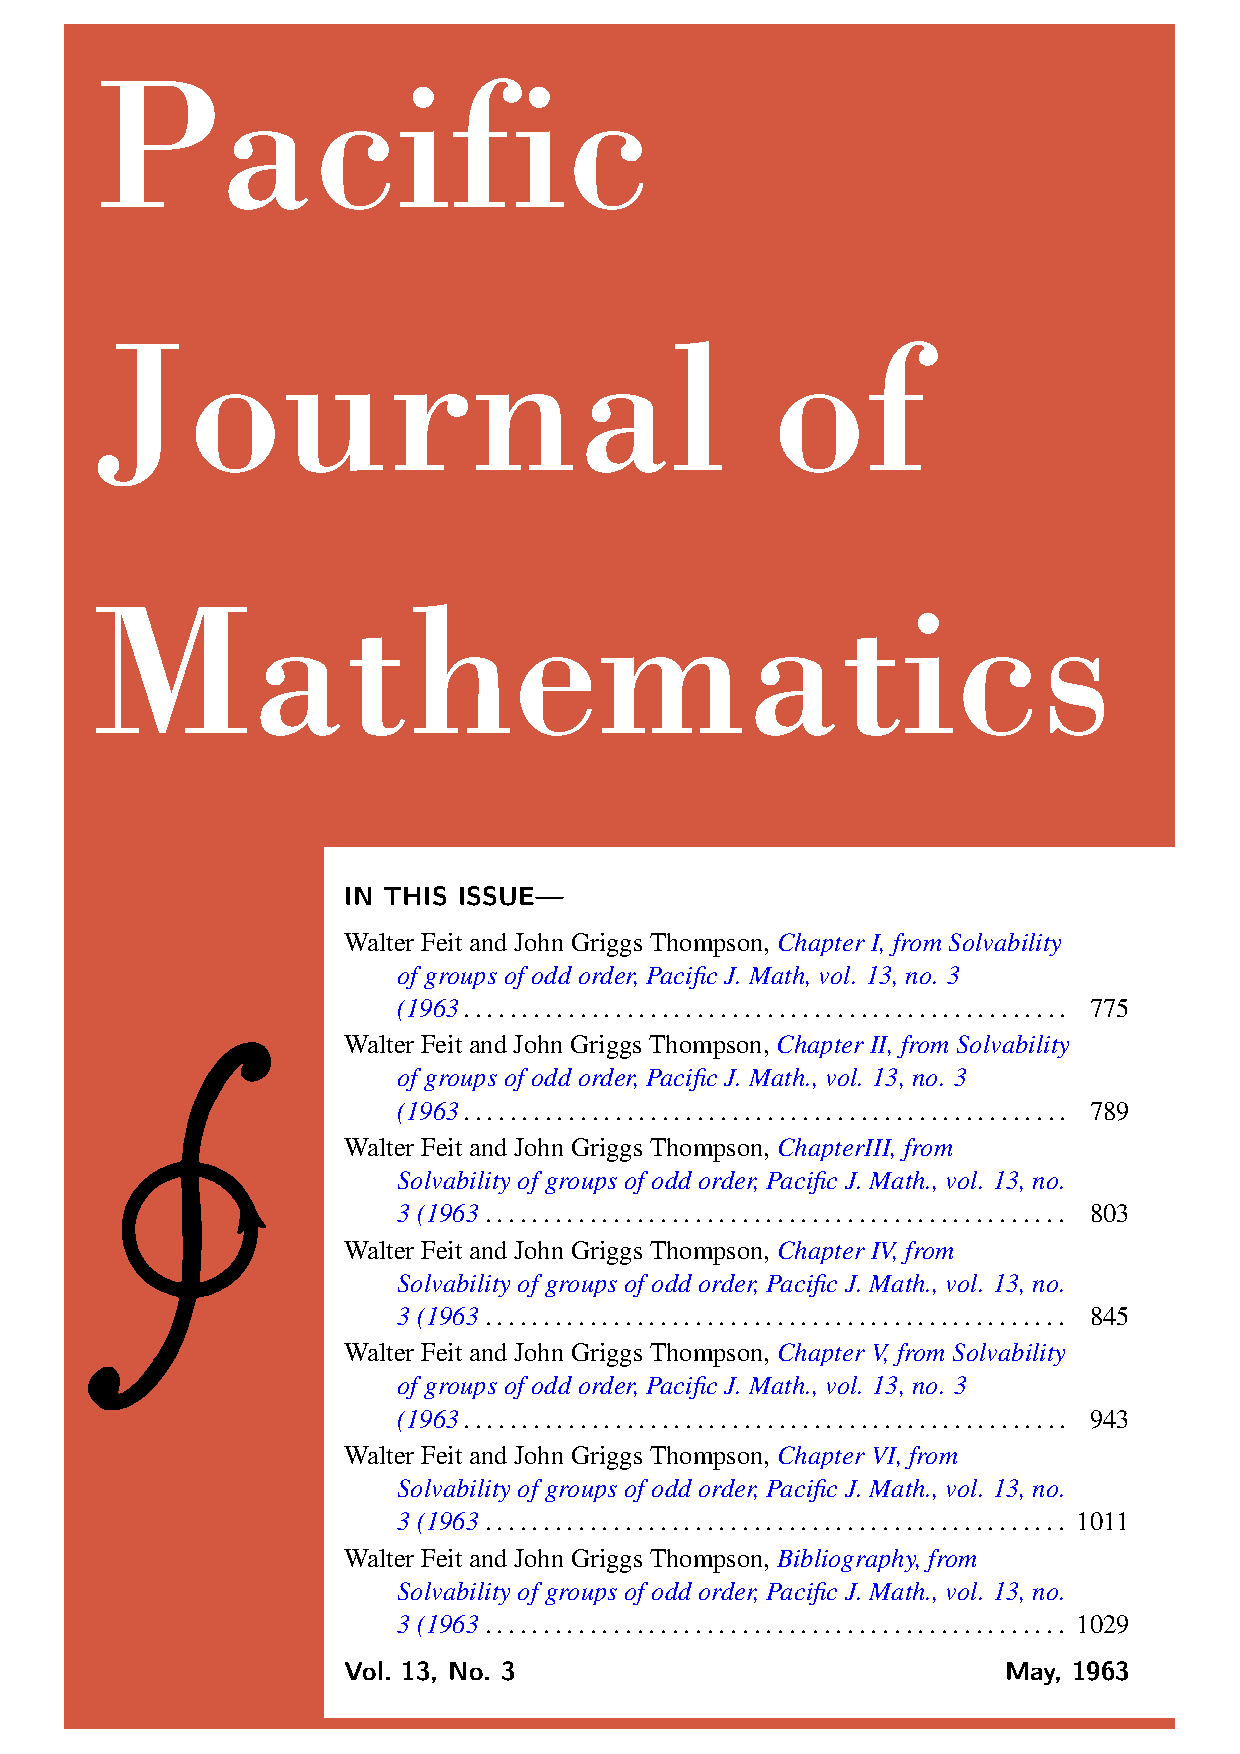
\includegraphics[scale=0.2]{FeitThompson.pdf}
    \caption{The proof of the Feit--Thompson theorem occupies a full volume of 
the Pacific Journal of Mathematics.}
    \label{fig:FeitThompson}
\end{figure}

The Feit--Thompson theorem is one of the starting points
of the classification of finite simple groups (CFSG). 
This classification is one
of the deepest theorems 
of the 20th century. The proof consists of tens of thousands 
of pages in several hundred journal articles written 
by about 100 authors, published mostly between 1955 and 2004.

\begin{theorem}[CFSG]
\index{Classification of simple groups}
\label{thm:CFSG}
Let $G$ be a finite simple group. Then $G$ lies in one (or more) 
of the following families:
\begin{enumerate}
    \item Cyclic groups of prime order.
    \item $\Alt_n$ for $n\geq5$.
    \item Finite groups of Lie type.
    \item 26 sporadic simple groups.
\end{enumerate}
\end{theorem}

Groups of Lie type are finite analogs of simple Lie groups, such as 
$\SL_n(\C)$. A typical example
of a finite simple group of Lie type is
$\PSL_n(p)$ for some prime number $p$, which is defined
as $\SL_n(p)$ over its center. 

The \emph{sporadic simple groups} are 26 groups that do not follow a systematic pattern. 
The first five of the sporadic groups were discovered by Mathieu in the 1860s, and the other 21 
were found between 1965 and 1975.
Several of these groups were predicted to exist before they were constructed, sometimes
just knowing their character tables! 
The full list of sporadic simple groups is as follows:
\begin{itemize}
\item Mathieu groups $M_{11}$, $M_{12}$, $M_{22}$, $M_{23}$ and $M_{24}$.
\item Janko groups $J_1$, $J_2$, $J_3$ and $J_4$.
\item Conway groups $Co_1$, $Co_2$ and $Co_3$.
\item Fischer groups $Fi_{22}$, $Fi_{23}$ and $Fi_{24}$. 
\item Higman–Sims group $HS$.
\item McLaughlin group $McL$.
\item Held group $He$.
\item Rudvalis group $Ru$.
\item Suzuki group $Suz$.
\item O'Nan group $ON$.
\item Harada–Norton group $HN$.
\item Lyons group $Ly$.
\item Thompson group $Th$.
\item Baby Monster group $B$.
\item Monster group $M$.
\end{itemize}

Mathieu groups can be realized 
as automorphism groups of certain very complicated
combinatorial structures known as \emph{Steiner systems}. 
A concrete example: 
\[
M_{11}=\langle (123456789\,10\,11), (37\,11\,8)(4\,10\,56)\rangle,
\]
which is a subgroup of $\Sym_{11}$ of order 7920. The group
$M_{11}$ contains ten irreducible characters, so the
character table of $M_{11}$ is essentially a $10\times 10$ matrix. Let us
use the computer software \lstinline{GAP} 
to see the character table:

\begin{lstlisting}
gap> Display(CharacterTable("M11"));
M11

      2  4  4  1  3  .  1  3  3   .   .
      3  2  1  2  .  .  1  .  .   .   .
      5  1  .  .  .  1  .  .  .   .   .
     11  1  .  .  .  .  .  .  .   1   1

        1a 2a 3a 4a 5a 6a 8a 8b 11a 11b
     2P 1a 1a 3a 2a 5a 3a 4a 4a 11b 11a
     3P 1a 2a 1a 4a 5a 2a 8a 8b 11a 11b
     5P 1a 2a 3a 4a 1a 6a 8b 8a 11a 11b
    11P 1a 2a 3a 4a 5a 6a 8a 8b  1a  1a

X.1      1  1  1  1  1  1  1  1   1   1
X.2     10  2  1  2  . -1  .  .  -1  -1
X.3     10 -2  1  .  .  1  A -A  -1  -1
X.4     10 -2  1  .  .  1 -A  A  -1  -1
X.5     11  3  2 -1  1  . -1 -1   .   .
X.6     16  . -2  .  1  .  .  .   B  /B
X.7     16  . -2  .  1  .  .  .  /B   B
X.8     44  4 -1  . -1  1  .  .   .   .
X.9     45 -3  .  1  .  . -1 -1   1   1
X.10    55 -1  1 -1  . -1  1  1   .   .

A = E(8)+E(8)^3
  = Sqrt(-2) = i2
B = E(11)+E(11)^3+E(11)^4+E(11)^5+E(11)^9
  = (-1+Sqrt(-11))/2 = b11
\end{lstlisting}

Thus the character table of the Mathieu group $M_{11}$ is
given by
\begin{center}
		\begin{tabular}{|c|cccccccccc|}
			\hline
			$\chi_{1}$ & 1 & 1 & 1 & 1 & 1 & 1 & 1 & 1 & 1 & 1\tabularnewline
			$\chi_{2}$ & 10 & 2 & 1 & 2 & 0 & -1 & 0 & 0 & -1 & -1 \tabularnewline
			$\chi_{3}$ & 10 & -2 & 1 & 0 & 0 & 1 & $\alpha$ & $-\alpha$ & -1 & -1\tabularnewline
		    $\chi_{4}$ & 10 & -2 & 1 & 0 & 0 & 1 & $-\alpha$ & $\alpha$ & -1 & -1\tabularnewline
		    $\chi_{5}$ & 11 & 3 & 2 &-1 & 1 & 0 & -1 & -1 & 0 & 0\tabularnewline
			$\chi_{6}$ & 16 & 0 & -2 & 0 & 1 & 0 & 0 & 0 & $\beta$ & $1/\beta$\tabularnewline
			$\chi_{7}$ & 16 & 0 & -2 & 0 & 1 & 0 & 0 & 0 & $1/\beta$ & $\beta$\tabularnewline
			$\chi_{8}$ & 44 & 4 &-1 & 0 &-1 & 1 & 0 & 0 & 0 & 0\tabularnewline
			$\chi_{9}$ & 45 & -3 & 0 & 1 & 0 & 0 &-1 &-1 &  1 & 1\tabularnewline
			$\chi_{10}$ & 55 & -1 & 1 & -1 & 0 & -1 & 1 & 1 & 0 & 0\tabularnewline
			\hline
		\end{tabular}    
\end{center}
where $\alpha=\sqrt{-2}$ and $\beta=\frac{-1-\sqrt{-11}}{2}$. 

The largest sporadic simple group is the \emph{Monster group} $M$ and has order
\[
808017424794512875886459904961710757005754368000000000, 
\]
which is roughly $8\times 10^{53}$. 
The monster group was predicted by Fischer and Griess. 
Griess proved the existence of the Monster group, realizing it as
the automorphism group of a certain space of dimension 196884. 
The group $M$ can be represented as
a subgroup of $\GL_{196883}(\C)$. It has 194 conjugacy classes, so 
the character table is a $194\times 194$ array. 

\begin{problem}
    Formalize the proof of Theorem \ref{thm:CFSG} in a proof assistant. 
\end{problem}

It is precisely due to the vastness of the theorem’s proof, that it is very suitable for formalization. Currently, only mathematicians with an extremely deep understanding of the subject can understand parts of the proof. 
By formalizing the proof in a proof assistant such as \lstinline{Coq} or \lstinline{Lean}, 
the complete proof could be verified at once. 